\documentclass[12pt]{article}
\usepackage{amsmath}
\usepackage{amsfonts}
\usepackage{graphicx}


\title{Image processing: A quick reference sheet for the exam}
\author{by Tom T. Doodle}

\begin{document}
\maketitle
\newpage
\tableofcontents
\newpage

\section{Introduction}
	This document is done in order to describe the general concepts
	that has been covered in the course, and also provide answers to
	some common exam questions. The content is shamelessly ripped from
	various sources, which is indicated at the start of a section
	or paragraph.\\
	\\	
	Guide:
	\begin{description}
		\item[[W]] Wikipedia
		\item[[L]] Lecture notes
		\item[[E]] Exam
		\item[[B]] Course Book
		\item[[O]] Other
	\end{description}
	
%	
%%%%%%%%%%%%%%%%%%%%%%%%%%%%%%%%%%%%%%%%%%%%%%%%%%%%%%%%%%%%%%%%%%%%%%%%%%%%%%%%%%%%%%%%%%%%%%%%%%%%%
%
\section{Noise}
	\subsection{General concepts}
	\subsubsection{What is noise?}
	
	[W] Image noise is random (not present in the object imaged) variation of brightness or
	color information in images, and is usually an aspect of electronic noise. It can be
	produced by the sensor and circuitry of a scanner or digital camera. Image noise can
	also originate in film grain and in the unavoidable shot noise of an ideal photon 
	detector. Image noise is an undesirable by-product of image capture that adds spurious 
	and extraneous information.\\
	
	The original meaning of "noise" was and remains "unwanted signal"; unwanted electrical
	fluctuations in signals received by AM radios caused audible acoustic noise ("static").
	By analogy unwanted electrical fluctuations themselves came to be known as "noise". 
	Image noise is, of course, inaudible.\\

	The magnitude of image noise can range from almost imperceptible specks on a digital 
	photograph taken in good light, to optical and radioastronomical images that are almost 
	entirely noise, from which a small amount of information can be derived by sophisticated 
	processing (a noise level that would be totally unacceptable in a photograph since it 
	would be impossible to determine even what the subject was).
	
	\subsection{Various types of noise}
	
	\subsubsection{Salt and pepper noise}
	[W] Salt-and-pepper noise is a form of noise sometimes seen on images. It presents itself as 
	sparsely occurring white and black pixels. An effective noise reduction method for this 
	type of noise is a \textbf{median filter} or a morphological filter. For reducing either salt 
	noise or pepper noise, but not both, a contraharmonic mean filter can be effective.
	\begin{figure}[h!]
		\centering
		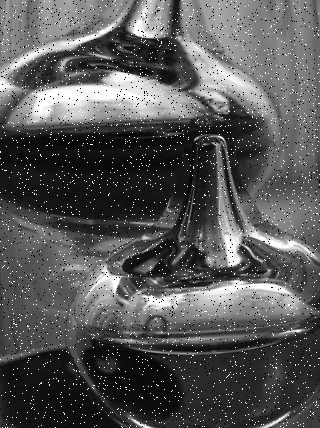
\includegraphics[width=0.5\textwidth]{img/Noise_salt_and_pepper.png}
		\caption{Example of salt and pepper noise}		
		\label{fig:salt_and_pepper}
	\end{figure}
	
	\subsubsection{Gaussian noise}
	[W] Gaussian noise is statistical noise having a probability density function (PDF) equal to 
	that of the normal distribution, which is also known as the Gaussian distribution. In other
	words, the values that the noise can take on are Gaussian-distributed.
	
	\subsubsection{Additive}
	TODO
	\subsubsection{Multiplicative}
	In signal processing, the term multiplicative noise refers to an unwanted random signal that 
	gets multiplied into some relevant signal during capture, transmission, or other processing.
	\subsubsection{Exponential}
	TODO
	
	\subsection{Colors of noise}
	\subsubsection{White noise}
	[W] White noise is a signal (or process), named by analogy to white light, with a flat frequency
	spectrum when plotted as a linear function of frequency (e.g., in Hz). In other words, the signal 
	has equal power in any band of a given bandwidth (power spectral density) when the bandwidth is 
	measured in Hz. 
	\subsubsection{Pink noise}
	TODO
	\subsubsection{Blue noise}
	[W] In computer graphics, the term "blue noise" is sometimes used more loosely as any noise with 
	minimal low frequency components and no concentrated spikes in energy. This can be good noise for dithering.
%	
%%%%%%%%%%%%%%%%%%%%%%%%%%%%%%%%%%%%%%%%%%%%%%%%%%%%%%%%%%%%%%%%%%%%%%%%%%%%%%%%%%%%%%%%%%%%%%%%%%%%%
%	
\section{Filters}
	
	\subsection{Median filter}
	\subsubsection{Description}
	[W] In signal processing, it is often desirable to be able to perform some kind of noise 
	reduction on an image or signal. The median filter is a nonlinear digital filtering 
	technique, often used to remove noise. Such noise reduction is a typical pre-processing 
	step to improve the results of later processing (for example, edge detection on an image). 
	Median filtering is very widely used in digital image processing because, under certain 
	conditions, it preserves edges while removing noise.
	
	\subsubsection{Algorithm description}
	[O] Like the mean filter, the median filter considers each pixel in the image in turn and 
	looks at its nearby neighbors to decide whether or not it is representative of its surroundings.\\
	\\
	Instead of simply replacing the pixel value with the mean of neighboring pixel values, it replaces 
	it with the median of those values. The median is calculated by first sorting all the pixel values 
	from the surrounding neighborhood into numerical order and then replacing the pixel being considered 
	with the middle pixel value. (If the neighborhood under consideration contains an even number of 
	pixels, the average of the two middle pixel values is used.)\\
	\\
	\textbf{Why use median instead of mean:}
	\begin{itemize}
	
	\item The median is a more robust average than the mean and so a single very unrepresentative pixel
	in a neighborhood will not affect the median value significantly.

    \item Since the median value must actually be the value of one of the pixels in the neighborhood, 
    the median filter does not create new unrealistic pixel values when the filter straddles an edge. 
    For this reason the median filter is much better at preserving sharp edges than the mean filter. 
	\end{itemize}

	\subsection{Mean filter}
	[O] The idea of mean filtering is simply to replace each pixel value in an image with the 
	mean (`average') value of its neighbors, including itself. This has the effect of eliminating 
	pixel values which are unrepresentative of their surroundings.\\
	\\	
	\textbf{Problems with mean filtering:}
	\begin{itemize}
		\item A single pixel with a very unrepresentative value can significantly affect 
		the mean value of all the pixels in its neighborhood. 
		\item When the filter neighborhood straddles an edge, the filter will interpolate 
		new values for pixels on the edge and so will blur that edge. This may be a problem
		if sharp edges are required in the output. 
	\end{itemize}
	Both of these problems are tackled by the median filter, which is often a better filter 
	for reducing noise than the mean filter, but it takes longer to compute. 
%	
%%%%%%%%%%%%%%%%%%%%%%%%%%%%%%%%%%%%%%%%%%%%%%%%%%%%%%%%%%%%%%%%%%%%%%%%%%%%%%%%%%%%%%%%%%%%%%%%%%%%%
%	
\section{Image sharpening}
	TODO
	\subsection{Edge detection}
	TODO
	\subsection{High Boosting}
	TODO	
%	
%%%%%%%%%%%%%%%%%%%%%%%%%%%%%%%%%%%%%%%%%%%%%%%%%%%%%%%%%%%%%%%%%%%%%%%%%%%%%%%%%%%%%%%%%%%%%%%%%%%%%
%	
\section{Image histograms}
	\subsection{Histogram equalization}
	[W] This method usually increases the global contrast of many images, especially when the usable data
	 of the image is represented by close contrast values. Through this adjustment, the intensities 
	 can be better distributed on the histogram. This allows for areas of lower local contrast to gain 
	 a higher contrast. Histogram equalization accomplishes this by effectively spreading out the most 
	 frequent intensity values.\\
	 \\
	The method is useful in images with backgrounds and foregrounds that are both bright or both dark. 
	In particular, the method can lead to better views of bone structure in x-ray images, and to 
	better detail in photographs that are over or under-exposed. A key advantage of the method is that 
	it is a fairly straightforward technique and an invertible operator. So in theory, if the 
	histogram equalization function is known, then the original histogram can be recovered. The 
	calculation is not computationally intensive. A disadvantage of the method is that it is 
	indiscriminate. It may increase the contrast of background noise, while decreasing the usable 
	signal.
	\begin{figure}[h!]
		\centering
		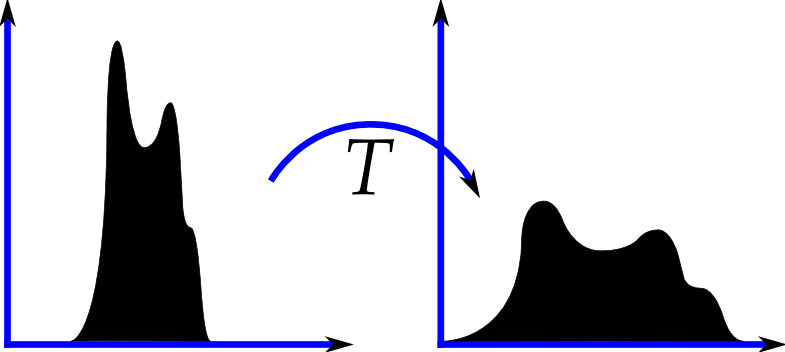
\includegraphics[width=0.5\textwidth]{img/histogram_equalization.png}
		\caption{Example of histogram equalization}		
		\label{fig:histeq}
	\end{figure}
	
	\subsection{Histogram matching}
	[W] It is possible to use histogram matching to balance detector responses as a relative detector 
	calibration technique. It can be used to normalize two images, when the images were acquired at 
	the same local illumination (such as shadows) over the same location, but by different sensors, 
	atmospheric conditions or global illumination.
%	
%%%%%%%%%%%%%%%%%%%%%%%%%%%%%%%%%%%%%%%%%%%%%%%%%%%%%%%%%%%%%%%%%%%%%%%%%%%%%%%%%%%%%%%%%%%%%%%%%%%%%
%	
\section{Wavelets}
	TODO
%	
%%%%%%%%%%%%%%%%%%%%%%%%%%%%%%%%%%%%%%%%%%%%%%%%%%%%%%%%%%%%%%%%%%%%%%%%%%%%%%%%%%%%%%%%%%%%%%%%%%%%%
%
\section{Image compression}
	TODO
%	
%%%%%%%%%%%%%%%%%%%%%%%%%%%%%%%%%%%%%%%%%%%%%%%%%%%%%%%%%%%%%%%%%%%%%%%%%%%%%%%%%%%%%%%%%%%%%%%%%%%%%
%	
\section{Old exams}
	TODO	
\end{document}